\documentclass[../../../../main.tex]{subfiles}
\begin{document}

\begin{flushright}
\footnotesize\textit{【自動文字起こし・要確認】}
\end{flushright}

\noindent
$\triangleright$ まず、楕円, 双曲線の図形的定義での書き方.

\begin{framed}
\noindent
\textbf{[楕円]}\\
$\overline{AP} + \overline{BP} = 2a$ の時、右のようになる。
\[
\frac{x^2}{a^2} + \frac{y^2}{a^2-c^2} = 1
\]
$\star$ まず、$a$ から手前的に端点をとる。\\
$\longrightarrow$ $c, a$ から $b$ をキメル

\begin{center}
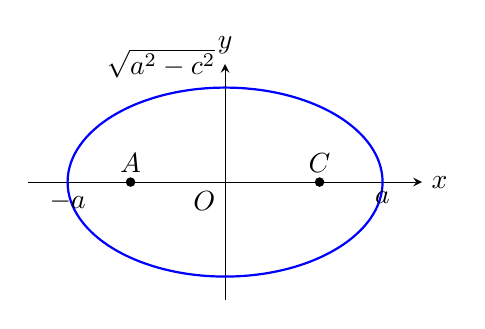
\begin{tikzpicture}[scale=1.0, >=stealth]
  \draw[->] (-2.5,0) -- (2.5,0) node[right] {$x$};
  \draw[->] (0,-1.5) -- (0,1.5) node[above] {$y$};
  \draw[thick, blue] (0,0) ellipse (2cm and 1.2cm);
  \filldraw (-1.2,0) circle (1.5pt) node[above] {$A$} (1.2,0) circle (1.5pt) node[above] {$C$};
  \node[below left] at (0,0) {$O$};
  \node[below] at (-2,0) {$-a$};
  \node[below] at (2,0) {$a$};
  \node[above left] at (0,1.2) {$\sqrt{a^2-c^2}$};
\end{tikzpicture}
\end{center}
\end{framed}

\begin{framed}
\noindent
\textbf{[双曲線]}\\
$|\overline{AP} - \overline{BP}| = 2a$ の時、右のようになる。
\[
\frac{x^2}{a^2} - \frac{y^2}{c^2-a^2} = 1
\]
$\star$ $a$ から端点 $\to$ $c, a$ から $b$\\
$\longrightarrow$ 漸近線 $\frac{x}{a} \pm \frac{y}{\sqrt{c^2-a^2}} = 0$

\begin{center}
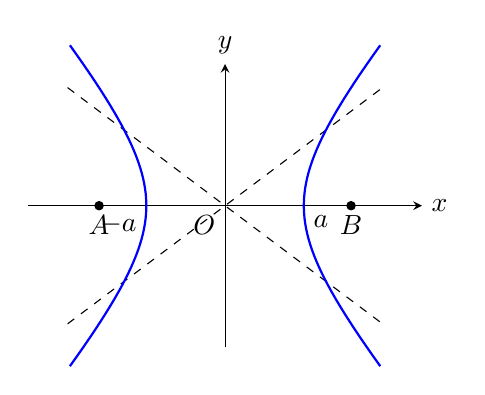
\begin{tikzpicture}[scale=1.0, >=stealth]
  \draw[->] (-2.5,0) -- (2.5,0) node[right] {$x$};
  \draw[->] (0,-1.8) -- (0,1.8) node[above] {$y$};
  \draw[dashed] (-2,-1.5) -- (2,1.5);
  \draw[dashed] (-2,1.5) -- (2,-1.5);
  \draw[thick, blue, domain=-1.3:1.3, samples=50] plot ({1*cosh(\x)}, {1.2*sinh(\x)});
  \draw[thick, blue, domain=-1.3:1.3, samples=50] plot ({-1*cosh(\x)}, {1.2*sinh(\x)});
  \filldraw (-1.6,0) circle (1.5pt) node[below] {$A$} (1.6,0) circle (1.5pt) node[below] {$B$};
  \node[below left] at (0,0) {$O$};
  \node[below left] at (-1,0) {$-a$};
  \node[below right] at (1,0) {$a$};
\end{tikzpicture}
\end{center}
\end{framed}

\newpage

\noindent
\textbf{[解]} $R(x,y)$ とおく。下図のように、$xy$ 平面を分割する。ただし $\square PTQS$ は正方形。

\begin{center}
\begin{tikzpicture}[scale=0.35, >=stealth]
  \draw[->] (-12,0) -- (12,0) node[right] {$x$};
  \draw[->] (0,-12) -- (0,12) node[above] {$y$};
  
  \filldraw (-9,-3) circle (3pt) node[left] {$P$};
  \filldraw (9,3) circle (3pt) node[right] {$Q$};
  \filldraw (-5,5) circle (2pt) node[left] {$L_4$};
  \filldraw (-5,-5) circle (2pt) node[left] {$L_3$};
  \filldraw (5,5) circle (2pt) node[right] {$L_1$};
  \filldraw (5,-5) circle (2pt) node[right] {$L_2$};

  \draw[dashed] (-5,-5) -- (-5,5) -- (5,5) -- (5,-5) -- cycle;
  \draw[dashed] (-9,-3) -- (9,3);
  \draw[thick] (-5,-5) -- (-5,5);
  \draw[thick] (5,-5) -- (5,5);

  \node at (0,0) {$C$};
  \node at (-9,5) {$A$};
  \node at (9,-5) {$B$};
\end{tikzpicture}
\end{center}

\noindent
左図で、斜線部は明らかに $d(P,R) = d(Q,R)$ とならない。\\
まず、$A, B$ について、$d(P,R) = d(Q,R)$ となるのは、線分 $PQ$ の垂直二等分線 $y = -3x$ 上である。 \quad \dots \text{①}

次に $C$ について、$\alpha,\beta$ のうち大きくない方を $\min\{\alpha,\beta\}$ と表すと、
\[
\begin{cases}
d(P,R) = \min \{ \overline{PL_3} + \overline{L_3R}, \overline{PL_4} + \overline{L_4R} \} \\
d(Q,R) = \min \{ \overline{QL_1} + \overline{L_1R}, \overline{QL_2} + \overline{L_2R} \}
\end{cases}
\quad \dots \text{②}
\]
である。$\overline{PL_3} = \overline{QL_1} = 2\sqrt{5}$, $\overline{PL_4} = \overline{QL_2} = 4\sqrt{5}$ \dots ③ だから,
\begin{align*}
\overline{PL_3} + \overline{L_3R} = \overline{PL_4} + \overline{L_4R} &\iff \overline{L_3R} - \overline{L_4R} = 2\sqrt{5} \quad \dots \text{④} \\
\overline{QL_1} + \overline{L_1R} = \overline{QL_2} + \overline{L_2R} &\iff \overline{L_1R} - \overline{L_2R} = 2\sqrt{5} \quad \dots \text{⑤}
\end{align*}
なので、$C$ をさらに、以下のように分割できる。

\begin{center}
\begin{tikzpicture}[scale=0.35, >=stealth]
  \draw[->] (-8,0) -- (8,0) node[right] {$x$};
  \draw[->] (0,-8) -- (0,8) node[above] {$y$};
  
  \draw[dashed] (-5,-5) -- (-5,5) -- (5,5) -- (5,-5) -- cycle;
  \node at (0,6) {$C_1$};
  \node at (0,-6) {$C_2$};
  \node at (0,0) {$C_3$};
  
  \draw[thick, domain=-5:5, samples=50] plot (\x, {sqrt(5*(1 + (\x+5)^2/20))});
  \draw[thick, domain=-5:5, samples=50] plot (\x, {-sqrt(5*(1 + (\x-5)^2/20))});
\end{tikzpicture}
\end{center}

\[
\begin{cases}
C_1 : d(P,R) = \overline{PL_4} + \overline{L_4R}, \quad d(Q,R) = \overline{QL_1} + \overline{L_1R} \\
C_2 : d(P,R) = \overline{PL_3} + \overline{L_3R}, \quad d(Q,R) = \overline{QL_2} + \overline{L_2R} \\
C_3 : d(P,R) = \overline{PL_3} + \overline{L_3R}, \quad d(Q,R) = \overline{QL_1} + \overline{L_1R}
\end{cases}
\]
境界は
\[
\frac{(x+5)^2}{20} - \frac{y^2}{5} = -1, \quad \frac{(x-5)^2}{20} - \frac{y^2}{5} = -1
\]

まず $C_1, C_2$ について、対称性から $C_1$ のみ考える。$C_1$ から
\[
d(P,R) = d(Q,R) \iff \overline{PL_4} + \overline{L_4R} = \overline{QL_1} + \overline{L_1R} \iff \overline{L_1R} - \overline{L_4R} = 2\sqrt{5}
\]
を満たす $R$ は、双曲線
\[
\frac{x^2}{5} - \frac{(y-5)^2}{20} = 1
\]
上にある。

$C_3$ について、④から、
\[
d(P,R) = d(Q,R) \iff \overline{PL_3} + \overline{L_3R} = \overline{QL_1} + \overline{L_1R} \iff \overline{L_3R} = \overline{L_1R}
\]
だから、$R$ は $\overline{L_1L_3}$ の垂直二等分線 $y = -x$ 上にある。

\bigskip
\noindent
以上まとめて、
\[
\begin{cases}
y = -3x & (|x| \ge 3) \\
y = -x & \left( |x| \le \frac{-5+4\sqrt{10}}{3} \right) \\
\frac{x^2}{5} - \frac{(y-5)^2}{20} = 1 & (C_1 \text{内}) \\
\frac{x^2}{5} - \frac{(y+5)^2}{20} = 1 & (C_2 \text{内})
\end{cases}
\]
だから、図示して下図太線部。

\begin{framed}
\begin{align*}
&y = -x \text{ と } \frac{x^2}{5} - \frac{(y-5)^2}{20} = 1 \text{ の交点は } 3x^2 - 10x - 45 = 0 \text{ の解} \\
&\text{共に } \left( \frac{5-4\sqrt{10}}{3}, \frac{-5+4\sqrt{10}}{3} \right) \text{ である。}
\end{align*}
\end{framed}

\begin{center}
\begin{tikzpicture}[scale=0.5, >=stealth]
  \draw[->] (-8,0) -- (8,0) node[right] {$x$};
  \draw[->] (0,-10) -- (0,10) node[above] {$y$};

  \draw[dashed] (-5,-5) -- (-5,5) -- (5,5) -- (5,-5) -- cycle;
  \draw[dashed, domain=-8:8] plot (\x, {-3*\x});
  \draw[dashed, domain=-7:7] plot (\x, {-\x});

  % Trajectory of R
  \draw[ultra thick, blue, domain=-8:-3] plot (\x, {-3*\x});
  \draw[ultra thick, blue, domain=3:8] plot (\x, {-3*\x});
  \draw[ultra thick, blue, domain=-2.55:2.55] plot (\x, {-\x});
  \draw[ultra thick, blue, domain=-3:-2.55, samples=50] plot (\x, {5 + sqrt(20*(1 + (\x)^2/5))});
  \draw[ultra thick, blue, domain=2.55:3, samples=50] plot (\x, {-5 - sqrt(20*(1 + (\x)^2/5))});

  \node[left] at (-3,9) {$y=-3x$};
  \node[right] at (3,-9) {$y=-3x$};
  \node[right] at (2,-2) {$y=-x$};
\end{tikzpicture}
\end{center}

\newpage

\end{document}
